\subsection{Graphics}

\subsubsection{Linux graphics driver}
In this assignment we use the Linux graphics driver to render our game on the LED screen of the
development board. The interface provided by the graphics driver is mainly by the system calls {\bf
  open}, {\bf write} and {\bf close} to the device file {\bf /dev/fb0}. To make things easier we use the
system call {\bf mmap} to memory map the entire file into userspace. This allows us to treat the LED
screen as a $320 * 240 * 3$ sized array of bytes inside our application. Writing to this array
causes the screen to be updated.\\
\\
The format of the screen is $320 * 240$ pixels, where each pixel contains 8 bits per color. The
colors are as usually {\it Red}, {\it Green} and {\it Blue}. This results in a dynamic range of 16 581
375 possible colors.

\subsubsection{Graphics module}
The graphics of the game is contained within the /graphics folder. Here the {\bf Screen} object is
responsible for communication with the framebuffer through the {\bf /dev/fb0} file. The {\bf Canvas}
object holds an array of {\bf Shape} objects. It has a method called {\bf CanvasPaint} where it
renders the screen in an 320x240 {\bf Pixel} array contained within the {\bf Screen}. When the whole
array has been updated the {\bf Canvas} object ask the {\bf Screen} object to copy the contents of
its internal buffer to the framebuffer. This causes the LED screen on the device to be updated. The
reason that we use an internal buffer inside the {\bf Screen} object is that if we let the canvas
object write to the actual frame buffer the rendering on the screen will cause a flicker effect. By
updating the whole frame buffer at once this effect is not seen by the naked eye.\\
\\
All graphical objects inherits their main structure of the {\bf Shape} object. The most important
part is the {\bf paint} method which {\bf Canvas} uses to render all the objects on the internal buffer.

\begin{figure}[h]
  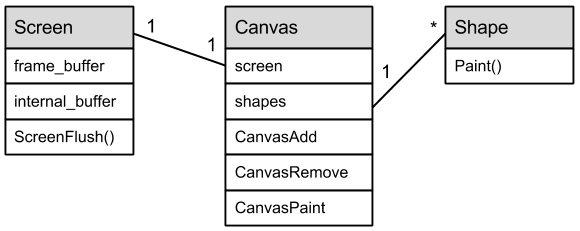
\includegraphics[width=350px]{graphics/graphics_UML.png}
  \caption{UML for the main part of the graphics module}
\end{figure}

\subsubsection{Bitmap Fileformat}
For all images the 24 bit version of the {\bf BMP}
(\footnote{http://en.wikipedia.org/wiki/BMP\_file\_format}{Bitmap file format}) was implemented.
This is done by the object {\bf Bitmap}, it is hidden behind the {\bf Image} object so that it is
easy to add more file formats. The reason that bitmap was chosen is that the 24 bit version
corresponds almost directly to the layout of the framebuffer, so the implementation was straight
forward.

%\caption{
\begin{table}[h]
  \centering
  \begin{tabular}{|c|c|}
    \hline
    16 bits&Signature \\
    \hline
    32 bits&File Size \\
    \hline
    16 bits&Reserved1 \\
    \hline
    16 bits&Reserved2 \\
    \hline
    32 bits&File Offset \\
    \hline
  \end{tabular}
  \qquad
  \begin{tabular}{|c|c|}
    \hline
    32 bits&Header size \\
    \hline
    32 bits&Image Width \\
    \hline
    32 bits&Image Height \\
    \hline
    & ...  \\
    \hline
  \end{tabular}
  \caption{Bitmap file header and first fields of DIB file header}
\end{table}
The file format is defined in the headerfile {\bf bitmap.h}. The only deviation from the Bitmap
standard is that we have defined the green color with values (55, 122, 46) to be transparant.

\subsubsection{Graphical objects}
Both objects for drawing lines and rectangles where used only in the testing of the graphics module
and are not used in the game. They serve as examples on how future development of graphical
objects can be done.
